\documentclass[a4paper,class=article,border=10pt,tikz]{standalone}
\usepackage{tikz}
\usetikzlibrary{snakes,calc,positioning,patterns,angles,quotes,decorations.pathmorphing,decorations.markings,through}
\usetikzlibrary{arrows,decorations,decorations.text}
\usepackage{rotating}
\usetikzlibrary{arrows,decorations,decorations.text}
\usetikzlibrary{patterns.meta,math}




\usepackage{siunitx}

\begin{document}

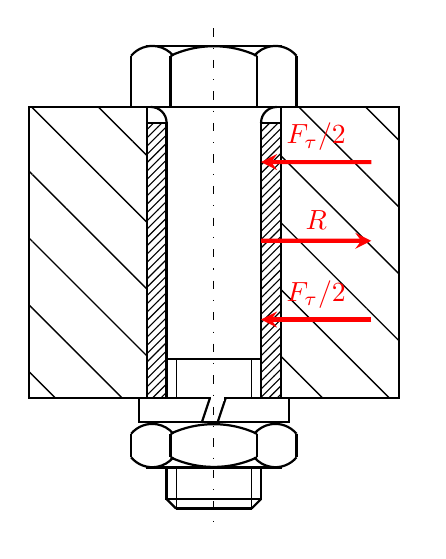
\begin{tikzpicture}

\tikzstyle{ground}=[fill,pattern=north east lines,draw=none,minimum width=0.75cm,minimum height=0.3cm]
\tikzstyle{close}=[draw=none,minimum width=0.75cm,minimum height=0.3cm]
\tikzstyle{spring}=[thick,decorate,decoration={zigzag,pre length=0.3cm,post length=0.3cm,segment length=0.3cm}]
\tikzstyle{force}=[>=stealth',ultra thick]

\coordinate (origo) at (0,0);


% Trzon śruby

\node (part2) [draw,outer sep=0pt,thick,minimum width=1.2cm, minimum height=0.5cm,anchor=north,label={right:{}}] at (origo) {};

\draw [ultra thin] ([xshift=0.12cm]part2.south west) -- ([xshift=0.12cm,yshift=0.5cm]part2.south west);
\draw [ultra thin] ([xshift=-0.12cm]part2.south east) -- ([xshift=-0.12cm,yshift=0.5cm]part2.south east);

% Łeb śruby

\draw[thick] ([yshift=3cm]part2.north west) arc (0:90:0.20cm);
\draw[thick] ([yshift=3cm]part2.north east) arc (180:90:0.20cm);

\draw [thick] ([xshift=-0.45cm,yshift=3.2cm]part2.north west) -- ([xshift=0.45cm,yshift=3.2cm]part2.north east);
\draw [thick] ([xshift=-0.26cm,yshift=3.97cm]part2.north west) -- ([xshift=0.26cm,yshift=3.97cm]part2.north east);

\draw[thick] ([xshift=-0.45cm,yshift=3.85cm]part2.north west) arc (140:40:0.35cm);
\draw[thick] ([xshift=0.45cm,yshift=3.85cm]part2.north east) arc (40:140:0.35cm);

\draw[thick] ([xshift=-0.55cm,yshift=3.85cm]part2.north) arc (115:65:1.3cm);

\draw [thick] ([xshift=-0.45cm,yshift=3.2cm]part2.north west) -- ([xshift=-0.45cm,yshift=3.85cm]part2.north west);
\draw [thick] ([xshift=0.45cm,yshift=3.2cm]part2.north east) -- ([xshift=0.45cm,yshift=3.85cm]part2.north east);

\draw [thick] ([xshift=-0.55cm,yshift=3.2cm]part2.north) -- ([xshift=-0.55cm,yshift=3.85cm]part2.north);
\draw [thick] ([xshift=0.55cm,yshift=3.2cm]part2.north) -- ([xshift=0.55cm,yshift=3.85cm]part2.north);

% Tuleja

\node (part3) [draw,pattern=north east lines,outer sep=0pt,thick,minimum width=0.25cm, minimum height=3.5cm,anchor=north,label={right:{}}] at ([xshift=-0.125cm,yshift=3cm]part2.north west) {};

\node (part4) [draw,pattern=north east lines,outer sep=0pt,thick,minimum width=0.25cm, minimum height=3.5cm,anchor=north,label={right:{}}] at ([xshift=0.125cm,yshift=3cm]part2.north east) {};

% Guma

\node (part52) [draw,pattern={Lines[angle=-45,distance={0.6cm}, line width=0.5pt,xshift=0.2cm]},outer sep=0pt,thick,minimum width=1.5cm, minimum height=3.7cm,anchor=north,label={right:{}}] at ([xshift=-1.6cm,yshift=3.2cm]part2.north) {};

\node (part62) [draw,pattern={Lines[angle=-45,distance={0.6cm}, line width=0.5pt,xshift=0.2cm]},outer sep=0pt,thick,minimum width=1.5cm, minimum height=3.7cm,anchor=north,label={right:{}}] at ([xshift=1.6cm,yshift=3.2cm]part2.north) {};
% podkładka

\node (part8) [draw,outer sep=0pt,thick,minimum width=1.9cm, minimum height=0.3cm,anchor=north,label={right:{}}] at (part2.south) {};

\draw [thick] ([xshift=-0.05cm]part8.north) -- ([xshift=-0.15cm]part8.south);
\draw [thick] ([xshift=0.15cm]part8.north) -- ([xshift=0.05cm]part8.south);

\draw [white,ultra thick] ([xshift=-0.04cm]part8.north) -- ([xshift=0.13cm]part8.north);
\draw [white,ultra thick] ([xshift=-0.04cm]part8.north) -- ([xshift=0.13cm]part8.north);
\draw [white,ultra thick] ([xshift=-0.04cm]part8.north) -- ([xshift=0.13cm]part8.north);
\draw [white,ultra thick] ([xshift=-0.04cm]part8.north) -- ([xshift=0.13cm]part8.north);
\draw [white,ultra thick] ([xshift=-0.04cm]part8.north) -- ([xshift=0.13cm]part8.north);
\draw [white,ultra thick] ([xshift=-0.04cm]part8.north) -- ([xshift=0.13cm]part8.north);

% nakrętka

\draw[thick] ([xshift=-0.45cm,yshift=-0.45cm]part2.south west) arc (140:40:0.35cm);
\draw[thick] ([xshift=0.45cm,yshift=-0.45cm]part2.south east) arc (40:140:0.35cm);
\draw[thick] ([xshift=-0.55cm,yshift=-0.45cm]part2.south) arc (115:65:1.3cm);

\draw [thick] ([xshift=-0.55cm,yshift=-0.45cm]part2.south) -- ([xshift=-0.55cm,yshift=-0.75cm]part2.south);
\draw [thick] ([xshift=0.55cm,yshift=-0.45cm]part2.south) -- ([xshift=0.55cm,yshift=-0.75cm]part2.south);
\draw [thick] ([xshift=-0.45cm,yshift=-0.45cm]part2.south west) -- ([xshift=-0.45cm,yshift=-0.75cm]part2.south west);
\draw [thick] ([xshift=0.45cm,yshift=-0.45cm]part2.south east) -- ([xshift=0.45cm,yshift=-0.75cm]part2.south east);

\draw[thick] ([xshift=-0.45cm,yshift=-0.75cm]part2.south west) arc (-140:-40:0.35cm);
\draw[thick] ([xshift=0.45cm,yshift=-0.75cm]part2.south east) arc (-40:-140:0.35cm);
\draw[thick] ([xshift=-0.55cm,yshift=-0.75cm]part2.south) arc (-115:-65:1.3cm);

\draw [thick] ([xshift=-0.26cm,yshift=-0.88cm]part2.south west) -- ([xshift=0.26cm,yshift=-0.88cm]part2.south east);

% Trzon śruby pod nakrętką

\node (part7) [draw,outer sep=0pt,thick,minimum width=1.2cm, minimum height=0.4cm,anchor=north,label={right:{}}] at ([yshift=-0.88cm]part2.south) {};

\draw [thick] (part7.south west) -- ++ (0.12,-0.12);
\draw [thick] (part7.south east) -- ++ (-0.12,-0.12);
\draw [thick]  ([xshift=0.12cm,yshift=-0.12cm]part7.south west) -- ([xshift=-0.12cm,yshift=-0.12cm]part7.south east);

\draw [ultra thin] ([xshift=0.12cm,yshift=-0.12cm]part7.south west) -- ([xshift=0.12cm,yshift=0.4cm]part7.south west);
\draw [ultra thin] ([xshift=-0.12cm,yshift=-0.12cm]part7.south east) -- ([xshift=-0.12cm,yshift=0.4cm]part7.south east);

% Oś

\draw [thin, loosely dashdotted] ([yshift=4.2cm]part2.north) --([yshift=-0.4cm]part7.south);

% Siły
\pgfmathsetmacro{\Fvec}{0.5}
\draw [red,-stealth,line width=1.5] (2,0.5) -- ($(part2.north east)!\Fvec cm!90:(part2.north east)$) coordinate (f1vec) node[midway,above] {$F_{\tau}/2$};

\pgfmathsetmacro{\Fvec}{1.5}
\draw [red,-stealth,line width=1.5]($(part2.north east)!\Fvec cm!90:(part2.north east)$) -- (2,1.5) coordinate (f1vec) node[midway,above] {$R$};

\pgfmathsetmacro{\Fvec}{2.5}
\draw [red,-stealth,line width=1.5] (2,2.5) -- ($(part2.north east)!\Fvec cm!90:(part2.north east)$) coordinate (f1vec) node[midway,above] {$F_{\tau}/2$};


% \node (ft) at ($(origo.north) + (0.75,1)$) {$F(t)$};
    
\end{tikzpicture}



\end{document}
